\section{Auswertung}
\label{sec:auswertung}
In diesem Kapitel werden die aufgenommenen Messwerte ausgewertet.
\subsection{Kugelkonstante}
\label{sec:Kugelkonstante}
In diesem Kapitel soll die Kugelkonstante $K_{gross}$ der großen Kugel bestimmt werden.
\subsubsection{Viskosität von Wasser bei 20,5 °C}
\label{sec:viskositaet1}
Da $\eta$ eine Konstante ist wurde diese zunächst mit den Angaben für die kleine Kugel berechnet 
um anschließend auf die Kugelkonstante $K_{gross}$ der der großen Kugel schließen zu können.
\begin{center}
    $t_{klein}={15.650\pm0.021}\si[]{s}$\\
    $K_{klein}=(5.08\pm0.08)\times10^{-4} \frac{cm^2}{s^2}$\\
    $\rho_{klein}=(2.233\pm0.009) \frac{g}{cm^3}$\\
    $\rho_F=(0.998103\pm0.0002169)\frac{g}{cm^3}$
\end{center}
Um die Dichte $\rho_F$ zu erhalten wurden aus einer Wertetabelle die Dichten für 19,5 °C, 20,5°C und 21,5 °C abgelesen,
anschließend wurde die Differenz zwischen der Dichte bei 20,5 °C zu den Dichten bei 19,5°C und 21,5°C berechnet und
der größere Wert als  Fehler angenommen. Für die Zeit $t$ wurde über alle Messwerte nach \autoref{eq:Mittelwert} gemittelt 
und der zugehörige Fehler über \autoref{eq:mittelwertfehler} berechnet. Nach der Gesetzmäßigkeit \autoref{eq:eta}
folgt mit den oben genannten Werten sofort:
\begin{center}
    $\eta=(0.00982\pm0.00017\frac{g}{cm*s})=(0.00982\pm0.00017)\si[]{P}=(0.982\pm0.017)\si[]{mPa*s}$
\end{center}
Um den zugehörigen Fehler zu berechnen kam \autoref{eq:gaussfehler}, die Gaußsche-Fehlerfortpflanzung zum Einsatz,
dazu wurde \autoref{eq:eta} partiell nach jeder fehlerbehafteten Größe abgeleitet. Die Ableitungen lauten:
\begin{center}
    $\frac{\partial \eta}{\partial t}=K_{klein}\left(\rho_{klein}-\rho_F\right)$
\end{center} 
\begin{center}
    $\frac{\partial \eta}{\partial K_{klein}}=\left(\rho_{klein}-\rho_F\right)t$
\end{center}
\begin{center}
    $\frac{\partial \eta}{\partial \rho_{klein}}=K_{klein}t$
\end{center}
\begin{center}
    $\frac{\partial \eta}{\partial \rho_F}=-K_{klein}t$
\end{center}
Die Einheit [Pa*s] oder [mPa*s] bezeichnet die Pascalsekunde bzw. die Millipascalsekunde und ist die in der 
Literatur gebräuchliche und gesetzliche Einheit für die Viskosität. Poise [P] ist die im experimentellen Umfeld
passendere, jedoch nicht gesetzmäßge Einheit. Es gilt:
\begin{center}
    $1\frac{g}{cm*s}=1\si[]{P}=0.1\si[]{Pa}*s=100\si[]{mPa*s}$
\end{center} 
\subsubsection{Berechnung von $K_{gross}$}
\label{sec:kugelkonstante1}
Nun Kann $K_{gross}$ leicht über:
\begin{equation}
    \label{eq:Kgross}
    K_{gross}=\frac{\eta}{t_{gross}*(\rho_{gross}-\rho_F)}
\end{equation}
berechnet werde. Dazu werden folgende Werte benutzt:
\begin{center}
    $\eta=(0.00982\pm0.00017)\si[]{P}$\\
    $t_{gross}=(131.48\pm0.16)\si[]{s}$\\
    $\rho_{gross}=(2.229\pm0.008)\frac{g}{cm^3}$\\
    $\rho_{F}=(0.998103\pm0.0002169)\frac{g}{cm^3}$
\end{center}
Alle Werte wurden mit ihren Fehlern wie schon oben beschrieben ermittelt und fürhren zu folgendem Ergebnis:
\begin{center}
    $K_{gross}=(6.07\pm0.11)\times 10^{-5} \frac{cm^2}{s^2}$
\end{center}
Der entsprchende Fehler wurde auch hier über die Gaußsche-Fehlerfortpflanzung \autoref{eq:gaussfehler} berechnet,
dazu wurden die folgenden Ableitungen genutzt:
\begin{center}
    $\frac{\partial K_{gross}}{\partial \eta}=\dfrac{1}{\left(\rho_{gross}-\rho_F\right)t}$
\end{center}
\begin{center}
    $\frac{\partial K_{gross}}{\partial t}=\dfrac{\eta}{\left(\rho_F-\rho_{gross}\right)t^2}$
\end{center}
\begin{center}
    $\frac{\partial K_{gross}}{\partial \rho_{gross}}=-\dfrac{\eta}{t\left(\rho_{gross}-\rho_F\right)^2}$
\end{center}
\begin{center}
    $\frac{\partial K_{gross}}{\partial \rho_{F}}=\dfrac{\eta}{t\left(\rho_{gross}-\rho_F\right)^2}$
\end{center}

\subsection{Temperaturabhängige Viskosität}
\label{sec:viskositaet}
Da $K_{gross}$ jetzt bekannt ist kann als nächstes die temperaturabhängige Viskosität von Wasser bestimmt werden.
Dazu werden zu allen Temperaturen, bei denen eine Messung durchgefüht wurde, die Dichten mit ihrem Fehler nach dem
Vorgehen aus \autoref{sec:viskositaet1} bestimmt. Hier in \autoref{fig:dichten} sind sie gegen die Temperatur $T$ aufgetragen:
\begin{figure}
    \centering
    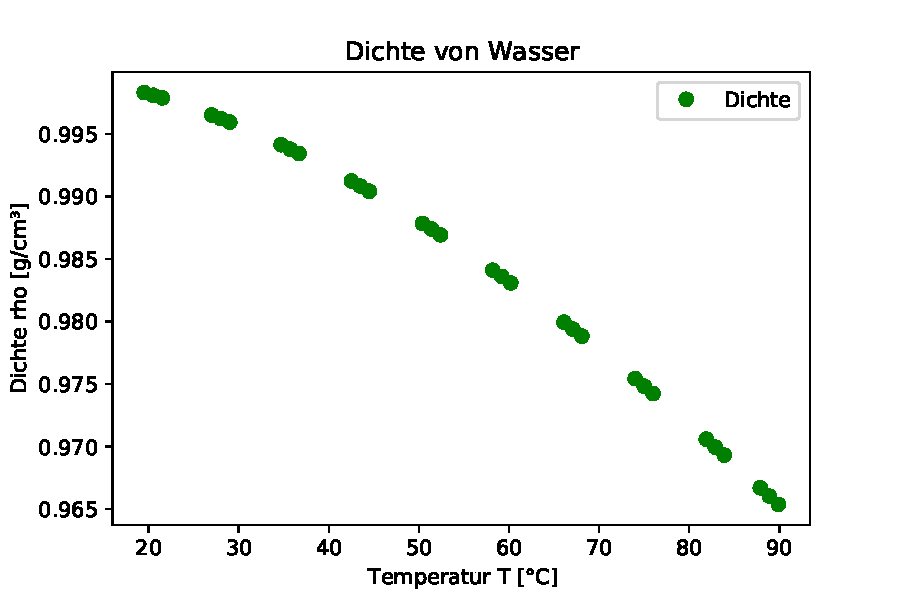
\includegraphics{dichten.pdf} %Name und datityp von dem Bild (am besten geht PDF einfach in Adobe Acrobat unter Werkzeuge -> PDF erstellen -> und dann ein belibiges Bild auswählen der macht aus allem ne PDF und es wird sofort passend skaliert. Die PDF muss dann im Ordner Viskosimeter gespeichert sein nicht in content)
    \caption{Temperaturabhängige Dichte von Wasser} % Bildunterschrift
    \label{fig:dichten}
  \end{figure}
  Es ergeben sich also folgende Werte zur Berechnung von $\eta(T)$:
  \begin{table}
    \centering
    \caption{Tempereaturen, Fallgeschindigkeiten und Dichten}
    \sisetup{table-format=1.2}
    \begin{tabular}{S[table-format=3.2] S S S S S S S  [table-format=3.2]}
      \toprule
      {$T$[°C]} & {$t$[Is]}& {$\rho_F$[$g/cm^3$]}\\
      \midrule
{$$20.500  \pm   1.0$$}  &   {$$94.267  \pm   30.115$$}  &   {$$0.998  \pm   0.000$$}\\
{$$28.000  \pm   1.0$$}  &   {$$82.300  \pm   22.168$$}  &   {$$0.996  \pm   0.000$$}\\
{$$35.700  \pm   1.0$$}  &   {$$73.900  \pm   15.596$$}  &   {$$0.994  \pm   0.000$$}\\
{$$43.500  \pm   1.0$$}  &   {$$67.300  \pm   9.726$$}   &   {$$0.991  \pm   0.000$$}\\
{$$51.400  \pm   1.0$$}  &   {$$64.133  \pm   5.198$$}   &   {$$0.987  \pm   0.000$$}\\
{$$59.200  \pm   1.0$$}  &   {$$61.500  \pm   0.946$$}   &   {$$0.984  \pm   0.001$$}\\
{$$67.100  \pm   1.0$$}  &   {$$59.067  \pm   3.280$$}   &   {$$0.979  \pm   0.001$$}\\
{$$75.000  \pm   1.0$$}  &   {$$57.733  \pm   7.049$$}   &   {$$0.975  \pm   0.001$$}\\
{$$82.900  \pm   1.0$$}  &   {$$57.367  \pm   10.428$$}  &  {$$ 0.970  \pm   0.001$$}\\
{$$88.900  \pm   1.0$$}  &   {$$58.067  \pm   12.588$$}  &  {$$ 0.966  \pm   0.001$$}\\
\bottomrule
    
    \end{tabular}
  \end{table}
\begin{center}
    $K_{gross}=(6.07\pm0.11)\times 10^{-5} \frac{cm^2}{s^2}$\\
    $\rho_{gross}=(2.229\pm0.008)\frac{g}{cm^3}$
\end{center}
Damit ergeben sich über \autoref{eq:eta} sofort folgende Werte für $\eta(T)$:

\begin{table}
    \centering
    \caption{Temperaturabhängigkeit der Viskosität}
    \sisetup{table-format=1.2}
    \begin{tabular}{S[table-format=3.2] S S S S    [table-format=3.2]}
      \toprule
      {$T$[°C]} & {$\eta$[P]}\\
      \midrule

{$$20.500  \pm   1.0$$}  &   {$$0.007  \pm   0.002$$}\\
{$$28.000  \pm   1.0$$}  &   {$$0.006  \pm   0.002$$}\\
{$$35.700  \pm   1.0$$}  &   {$$0.006  \pm   0.001$$}\\
{$$43.500  \pm   1.0$$}  &   {$$0.005  \pm   0.001$$}\\
{$$51.400  \pm   1.0$$}  &   {$$0.005  \pm   0.000$$}\\
{$$59.200  \pm   1.0$$}  &   {$$0.005  \pm   0.000$$}\\
{$$67.100  \pm   1.0$$}  &   {$$0.004  \pm   0.000$$}\\
{$$75.000  \pm   1.0$$}  &   {$$0.004  \pm   0.001$$}\\
{$$82.900  \pm   1.0$$}  &   {$$0.004  \pm   0.001$$}\\
{$$88.900  \pm   1.0$$}  &   {$$0.004  \pm   0.001$$}\\
\bottomrule
    
    \end{tabular}
  \end{table}
Die entsprechenden Fehler wurden wieder nach \autoref{eq:gaussfehler} berechnet, dazu konnten die Ableitungen aus
\autoref{sec:viskositaet1} wiederverwendet werden.
Diese Werte werden in \autoref{fig:viskositaet} grafisch dargestellt und mit einer Theoriekurve verglichen.
\begin{figure}
    \centering
    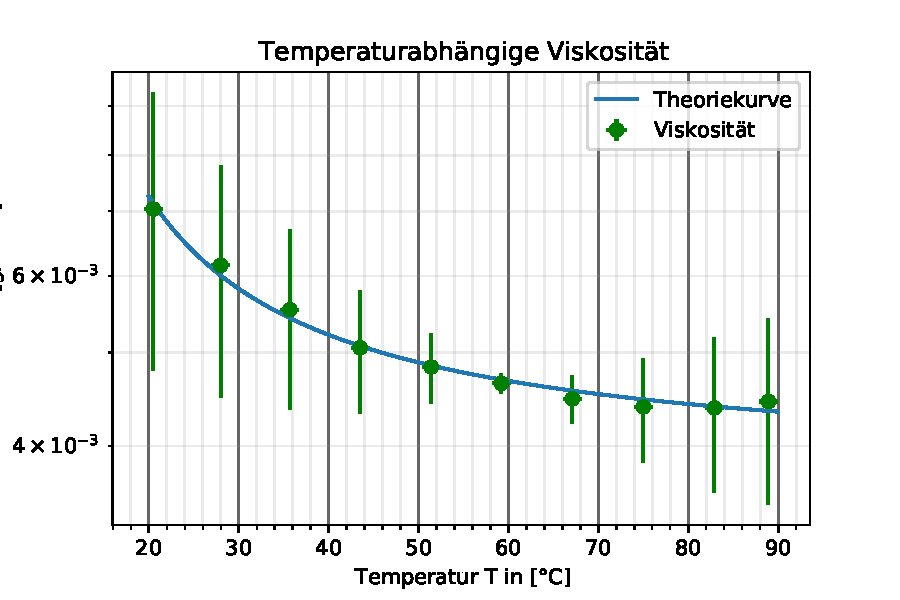
\includegraphics{Viskositaet.pdf} %Name und datityp von dem Bild (am besten geht PDF einfach in Adobe Acrobat unter Werkzeuge -> PDF erstellen -> und dann ein belibiges Bild auswählen der macht aus allem ne PDF und es wird sofort passend skaliert. Die PDF muss dann im Ordner Viskosimeter gespeichert sein nicht in content)
    \caption{Viskosität von Wasser in Abhängigkeit der Temperatur} % Bildunterschrift
    \label{fig:viskositaet}
  \end{figure}
  Die Theoriekurve folgt der Vorschrift \autoref{eq:theoriekurve} mit folgenden Koeffizienten:
  \begin{center}
      $A=0.004 \pm 0.000 g$\\
      $B=13.191 \pm 0.433\frac{1}{cm}$
  \end{center}